\section{Excitation towards $5s$ state}

The last part of this study, which is still in progress, is the simulation of the $5s\leftarrow 4s$ photo-excitation. 
Since the ($5s$) state is isotropic, we could address this problem with both a classical and a quantum description for potassium.

\subsection{Qualitative behavior and time scale}

The first element that can be compared between the two approaches is the behavior of the potassium. 
In both cases it is ejected after excitation within 200 fs (\citfig{fig:5S-pos}). 
This was actually highly predictable looking at the pair potential (\citfig{fig:DIM-5s-pot}): it shows a potential energy of 700 K over the dissociation level (and in an isotropic state all helium-potassium pairs interact with the same potential). Nevertheless, we see that the asymptotic K velocity is not the same  in quantum and classical description (\citfig{fig:5S-vel}). We will investigate this point in the following paragraph.

\begin{figure}[h!]
	\centering
	\begin{minipage}[c]{0.48\linewidth}
		% GNUPLOT: LaTeX picture with Postscript
\begingroup
  \makeatletter
  \providecommand\color[2][]{%
    \GenericError{(gnuplot) \space\space\space\@spaces}{%
      Package color not loaded in conjunction with
      terminal option `colourtext'%
    }{See the gnuplot documentation for explanation.%
    }{Either use 'blacktext' in gnuplot or load the package
      color.sty in LaTeX.}%
    \renewcommand\color[2][]{}%
  }%
  \providecommand\includegraphics[2][]{%
    \GenericError{(gnuplot) \space\space\space\@spaces}{%
      Package graphicx or graphics not loaded%
    }{See the gnuplot documentation for explanation.%
    }{The gnuplot epslatex terminal needs graphicx.sty or graphics.sty.}%
    \renewcommand\includegraphics[2][]{}%
  }%
  \providecommand\rotatebox[2]{#2}%
  \@ifundefined{ifGPcolor}{%
    \newif\ifGPcolor
    \GPcolortrue
  }{}%
  \@ifundefined{ifGPblacktext}{%
    \newif\ifGPblacktext
    \GPblacktextfalse
  }{}%
  % define a \g@addto@macro without @ in the name:
  \let\gplgaddtomacro\g@addto@macro
  % define empty templates for all commands taking text:
  \gdef\gplbacktext{}%
  \gdef\gplfronttext{}%
  \makeatother
  \ifGPblacktext
    % no textcolor at all
    \def\colorrgb#1{}%
    \def\colorgray#1{}%
  \else
    % gray or color?
    \ifGPcolor
      \def\colorrgb#1{\color[rgb]{#1}}%
      \def\colorgray#1{\color[gray]{#1}}%
      \expandafter\def\csname LTw\endcsname{\color{white}}%
      \expandafter\def\csname LTb\endcsname{\color{black}}%
      \expandafter\def\csname LTa\endcsname{\color{black}}%
      \expandafter\def\csname LT0\endcsname{\color[rgb]{1,0,0}}%
      \expandafter\def\csname LT1\endcsname{\color[rgb]{0,1,0}}%
      \expandafter\def\csname LT2\endcsname{\color[rgb]{0,0,1}}%
      \expandafter\def\csname LT3\endcsname{\color[rgb]{1,0,1}}%
      \expandafter\def\csname LT4\endcsname{\color[rgb]{0,1,1}}%
      \expandafter\def\csname LT5\endcsname{\color[rgb]{1,1,0}}%
      \expandafter\def\csname LT6\endcsname{\color[rgb]{0,0,0}}%
      \expandafter\def\csname LT7\endcsname{\color[rgb]{1,0.3,0}}%
      \expandafter\def\csname LT8\endcsname{\color[rgb]{0.5,0.5,0.5}}%
    \else
      % gray
      \def\colorrgb#1{\color{black}}%
      \def\colorgray#1{\color[gray]{#1}}%
      \expandafter\def\csname LTw\endcsname{\color{white}}%
      \expandafter\def\csname LTb\endcsname{\color{black}}%
      \expandafter\def\csname LTa\endcsname{\color{black}}%
      \expandafter\def\csname LT0\endcsname{\color{black}}%
      \expandafter\def\csname LT1\endcsname{\color{black}}%
      \expandafter\def\csname LT2\endcsname{\color{black}}%
      \expandafter\def\csname LT3\endcsname{\color{black}}%
      \expandafter\def\csname LT4\endcsname{\color{black}}%
      \expandafter\def\csname LT5\endcsname{\color{black}}%
      \expandafter\def\csname LT6\endcsname{\color{black}}%
      \expandafter\def\csname LT7\endcsname{\color{black}}%
      \expandafter\def\csname LT8\endcsname{\color{black}}%
    \fi
  \fi
    \setlength{\unitlength}{0.0500bp}%
    \ifx\gptboxheight\undefined%
      \newlength{\gptboxheight}%
      \newlength{\gptboxwidth}%
      \newsavebox{\gptboxtext}%
    \fi%
    \setlength{\fboxrule}{0.5pt}%
    \setlength{\fboxsep}{1pt}%
\begin{picture}(4752.00,2880.00)%
    \gplgaddtomacro\gplbacktext{%
      \csname LTb\endcsname%
      \put(682,782){\makebox(0,0)[r]{\strut{}$26$}}%
      \csname LTb\endcsname%
      \put(682,1481){\makebox(0,0)[r]{\strut{}$27$}}%
      \csname LTb\endcsname%
      \put(682,2180){\makebox(0,0)[r]{\strut{}$28$}}%
      \csname LTb\endcsname%
      \put(682,2879){\makebox(0,0)[r]{\strut{}$29$}}%
      \csname LTb\endcsname%
      \put(814,212){\makebox(0,0){\strut{}$0$}}%
      \csname LTb\endcsname%
      \put(1554,212){\makebox(0,0){\strut{}$0.2$}}%
      \csname LTb\endcsname%
      \put(2294,212){\makebox(0,0){\strut{}$0.4$}}%
      \csname LTb\endcsname%
      \put(3033,212){\makebox(0,0){\strut{}$0.6$}}%
      \csname LTb\endcsname%
      \put(3773,212){\makebox(0,0){\strut{}$0.8$}}%
      \csname LTb\endcsname%
      \put(4513,212){\makebox(0,0){\strut{}$1$}}%
    }%
    \gplgaddtomacro\gplfronttext{%
      \csname LTb\endcsname%
      \put(176,1655){\rotatebox{-270}{\makebox(0,0){\strut{}K relative position (\AA)}}}%
      \put(2663,-74){\makebox(0,0){\strut{}Time (ps)}}%
      \csname LTb\endcsname%
      \put(3922,1031){\makebox(0,0)[r]{\strut{}Classical}}%
      \csname LTb\endcsname%
      \put(3922,811){\makebox(0,0)[r]{\strut{}Quantum}}%
    }%
    \gplbacktext
    \put(0,0){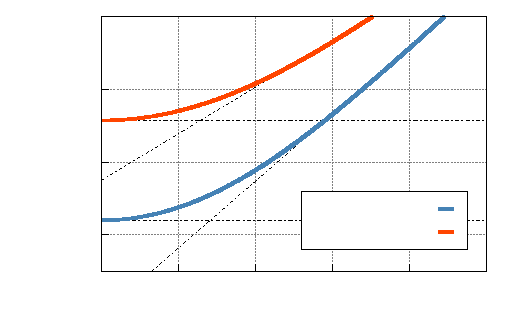
\includegraphics{5S-pos}}%
    \gplfronttext
  \end{picture}%
\endgroup

		\vspace{0.2\baselineskip}
		\caption{Distance between classical/quantum K and He$_N$ centers of mass as a function of time\label{fig:5S-pos}}
	\end{minipage}
\hfill
	\begin{minipage}[c]{0.48\linewidth}
		% GNUPLOT: LaTeX picture with Postscript
\begingroup
  \makeatletter
  \providecommand\color[2][]{%
    \GenericError{(gnuplot) \space\space\space\@spaces}{%
      Package color not loaded in conjunction with
      terminal option `colourtext'%
    }{See the gnuplot documentation for explanation.%
    }{Either use 'blacktext' in gnuplot or load the package
      color.sty in LaTeX.}%
    \renewcommand\color[2][]{}%
  }%
  \providecommand\includegraphics[2][]{%
    \GenericError{(gnuplot) \space\space\space\@spaces}{%
      Package graphicx or graphics not loaded%
    }{See the gnuplot documentation for explanation.%
    }{The gnuplot epslatex terminal needs graphicx.sty or graphics.sty.}%
    \renewcommand\includegraphics[2][]{}%
  }%
  \providecommand\rotatebox[2]{#2}%
  \@ifundefined{ifGPcolor}{%
    \newif\ifGPcolor
    \GPcolortrue
  }{}%
  \@ifundefined{ifGPblacktext}{%
    \newif\ifGPblacktext
    \GPblacktextfalse
  }{}%
  % define a \g@addto@macro without @ in the name:
  \let\gplgaddtomacro\g@addto@macro
  % define empty templates for all commands taking text:
  \gdef\gplbacktext{}%
  \gdef\gplfronttext{}%
  \makeatother
  \ifGPblacktext
    % no textcolor at all
    \def\colorrgb#1{}%
    \def\colorgray#1{}%
  \else
    % gray or color?
    \ifGPcolor
      \def\colorrgb#1{\color[rgb]{#1}}%
      \def\colorgray#1{\color[gray]{#1}}%
      \expandafter\def\csname LTw\endcsname{\color{white}}%
      \expandafter\def\csname LTb\endcsname{\color{black}}%
      \expandafter\def\csname LTa\endcsname{\color{black}}%
      \expandafter\def\csname LT0\endcsname{\color[rgb]{1,0,0}}%
      \expandafter\def\csname LT1\endcsname{\color[rgb]{0,1,0}}%
      \expandafter\def\csname LT2\endcsname{\color[rgb]{0,0,1}}%
      \expandafter\def\csname LT3\endcsname{\color[rgb]{1,0,1}}%
      \expandafter\def\csname LT4\endcsname{\color[rgb]{0,1,1}}%
      \expandafter\def\csname LT5\endcsname{\color[rgb]{1,1,0}}%
      \expandafter\def\csname LT6\endcsname{\color[rgb]{0,0,0}}%
      \expandafter\def\csname LT7\endcsname{\color[rgb]{1,0.3,0}}%
      \expandafter\def\csname LT8\endcsname{\color[rgb]{0.5,0.5,0.5}}%
    \else
      % gray
      \def\colorrgb#1{\color{black}}%
      \def\colorgray#1{\color[gray]{#1}}%
      \expandafter\def\csname LTw\endcsname{\color{white}}%
      \expandafter\def\csname LTb\endcsname{\color{black}}%
      \expandafter\def\csname LTa\endcsname{\color{black}}%
      \expandafter\def\csname LT0\endcsname{\color{black}}%
      \expandafter\def\csname LT1\endcsname{\color{black}}%
      \expandafter\def\csname LT2\endcsname{\color{black}}%
      \expandafter\def\csname LT3\endcsname{\color{black}}%
      \expandafter\def\csname LT4\endcsname{\color{black}}%
      \expandafter\def\csname LT5\endcsname{\color{black}}%
      \expandafter\def\csname LT6\endcsname{\color{black}}%
      \expandafter\def\csname LT7\endcsname{\color{black}}%
      \expandafter\def\csname LT8\endcsname{\color{black}}%
    \fi
  \fi
    \setlength{\unitlength}{0.0500bp}%
    \ifx\gptboxheight\undefined%
      \newlength{\gptboxheight}%
      \newlength{\gptboxwidth}%
      \newsavebox{\gptboxtext}%
    \fi%
    \setlength{\fboxrule}{0.5pt}%
    \setlength{\fboxsep}{1pt}%
\begin{picture}(4752.00,2880.00)%
    \gplgaddtomacro\gplbacktext{%
      \csname LTb\endcsname%
      \put(550,432){\makebox(0,0)[r]{\strut{}$0$}}%
      \csname LTb\endcsname%
      \put(550,840){\makebox(0,0)[r]{\strut{}$1$}}%
      \csname LTb\endcsname%
      \put(550,1248){\makebox(0,0)[r]{\strut{}$2$}}%
      \csname LTb\endcsname%
      \put(550,1656){\makebox(0,0)[r]{\strut{}$3$}}%
      \csname LTb\endcsname%
      \put(550,2063){\makebox(0,0)[r]{\strut{}$4$}}%
      \csname LTb\endcsname%
      \put(550,2471){\makebox(0,0)[r]{\strut{}$5$}}%
      \csname LTb\endcsname%
      \put(550,2879){\makebox(0,0)[r]{\strut{}$6$}}%
      \csname LTb\endcsname%
      \put(682,212){\makebox(0,0){\strut{}$0$}}%
      \csname LTb\endcsname%
      \put(1229,212){\makebox(0,0){\strut{}$2$}}%
      \csname LTb\endcsname%
      \put(1777,212){\makebox(0,0){\strut{}$4$}}%
      \csname LTb\endcsname%
      \put(2324,212){\makebox(0,0){\strut{}$6$}}%
      \csname LTb\endcsname%
      \put(2871,212){\makebox(0,0){\strut{}$8$}}%
      \csname LTb\endcsname%
      \put(3418,212){\makebox(0,0){\strut{}$10$}}%
      \csname LTb\endcsname%
      \put(3966,212){\makebox(0,0){\strut{}$12$}}%
      \csname LTb\endcsname%
      \put(4513,212){\makebox(0,0){\strut{}$14$}}%
    }%
    \gplgaddtomacro\gplfronttext{%
      \csname LTb\endcsname%
      \put(176,1655){\rotatebox{-270}{\makebox(0,0){\strut{}K velocity (\AA/ps)}}}%
      \put(2597,-74){\makebox(0,0){\strut{}Time (ps)}}%
      \csname LTb\endcsname%
      \put(3915,1031){\makebox(0,0)[r]{\strut{}Classical}}%
      \csname LTb\endcsname%
      \put(3915,811){\makebox(0,0)[r]{\strut{}Quantum}}%
    }%
    \gplbacktext
    \put(0,0){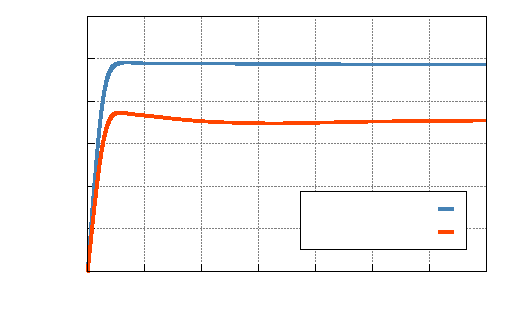
\includegraphics{5S-vel}}%
    \gplfronttext
  \end{picture}%
\endgroup

		\vspace{0.2\baselineskip}
		\caption{Velocity of classical/quantum K and He$_N$ as a function of time\newline{}\label{fig:5S-vel}}
	\end{minipage}
\end{figure}

\subsection{Strongly interacting neighbor helium atoms}

Let us consider a simple, impulsive  model, which has already been used in the past \cite{Her2012}. 
K interacts with $M$ neighboring He atoms. We assume that all the excitation energy $\Delta E$ (\textit{id est} excess energy with respect to the dissociation threshold) is converted into kinetic energy. 
We can write both energy and momentum conservation
\begin{align}
\frac{\vb{p}_\K^2}{2m\K}+\sum_\HE^M \cdot\frac{\vb{p}^2_{\HE}}{2m_\HE} &= \Delta E\\
\vb{p}_\K + \sum_\HE^M \cdot \vb{p}_\HE &= 0 
\end{align}
Then we make the following assumption: all He momentum are equal, this is quite a huge approximation but this model is simple. Then some basic algebra gives an expression for $M$
\begin{align}
\frac{\vb{p}_\K^2}{2m\K} &= \frac{M\cdot m_\HE}{m_K+M\cdot m_\HE} \Delta E \equiv \alpha \, \Delta E\\
M &= \frac{\alpha}{1-\alpha} \frac{m_\K}{m_\HE}
\end{align}

In order to probe different excitation energies we have to shift the initial position of the potassium at excitation time. 
In the classical description  of K we could study both diabatic or adiabatic helium density (\textit{with frozen or relaxed helium density for the new position)}, while the quantum case will only be discussed within the adiabatic approximation, but the diabatic one is being studied currently. 
\begin{figure}[h!]
\centering
\begin{minipage}[c]{0.48\linewidth}
\centering
		% GNUPLOT: LaTeX picture with Postscript
\begingroup
  \makeatletter
  \providecommand\color[2][]{%
    \GenericError{(gnuplot) \space\space\space\@spaces}{%
      Package color not loaded in conjunction with
      terminal option `colourtext'%
    }{See the gnuplot documentation for explanation.%
    }{Either use 'blacktext' in gnuplot or load the package
      color.sty in LaTeX.}%
    \renewcommand\color[2][]{}%
  }%
  \providecommand\includegraphics[2][]{%
    \GenericError{(gnuplot) \space\space\space\@spaces}{%
      Package graphicx or graphics not loaded%
    }{See the gnuplot documentation for explanation.%
    }{The gnuplot epslatex terminal needs graphicx.sty or graphics.sty.}%
    \renewcommand\includegraphics[2][]{}%
  }%
  \providecommand\rotatebox[2]{#2}%
  \@ifundefined{ifGPcolor}{%
    \newif\ifGPcolor
    \GPcolortrue
  }{}%
  \@ifundefined{ifGPblacktext}{%
    \newif\ifGPblacktext
    \GPblacktextfalse
  }{}%
  % define a \g@addto@macro without @ in the name:
  \let\gplgaddtomacro\g@addto@macro
  % define empty templates for all commands taking text:
  \gdef\gplbacktext{}%
  \gdef\gplfronttext{}%
  \makeatother
  \ifGPblacktext
    % no textcolor at all
    \def\colorrgb#1{}%
    \def\colorgray#1{}%
  \else
    % gray or color?
    \ifGPcolor
      \def\colorrgb#1{\color[rgb]{#1}}%
      \def\colorgray#1{\color[gray]{#1}}%
      \expandafter\def\csname LTw\endcsname{\color{white}}%
      \expandafter\def\csname LTb\endcsname{\color{black}}%
      \expandafter\def\csname LTa\endcsname{\color{black}}%
      \expandafter\def\csname LT0\endcsname{\color[rgb]{1,0,0}}%
      \expandafter\def\csname LT1\endcsname{\color[rgb]{0,1,0}}%
      \expandafter\def\csname LT2\endcsname{\color[rgb]{0,0,1}}%
      \expandafter\def\csname LT3\endcsname{\color[rgb]{1,0,1}}%
      \expandafter\def\csname LT4\endcsname{\color[rgb]{0,1,1}}%
      \expandafter\def\csname LT5\endcsname{\color[rgb]{1,1,0}}%
      \expandafter\def\csname LT6\endcsname{\color[rgb]{0,0,0}}%
      \expandafter\def\csname LT7\endcsname{\color[rgb]{1,0.3,0}}%
      \expandafter\def\csname LT8\endcsname{\color[rgb]{0.5,0.5,0.5}}%
    \else
      % gray
      \def\colorrgb#1{\color{black}}%
      \def\colorgray#1{\color[gray]{#1}}%
      \expandafter\def\csname LTw\endcsname{\color{white}}%
      \expandafter\def\csname LTb\endcsname{\color{black}}%
      \expandafter\def\csname LTa\endcsname{\color{black}}%
      \expandafter\def\csname LT0\endcsname{\color{black}}%
      \expandafter\def\csname LT1\endcsname{\color{black}}%
      \expandafter\def\csname LT2\endcsname{\color{black}}%
      \expandafter\def\csname LT3\endcsname{\color{black}}%
      \expandafter\def\csname LT4\endcsname{\color{black}}%
      \expandafter\def\csname LT5\endcsname{\color{black}}%
      \expandafter\def\csname LT6\endcsname{\color{black}}%
      \expandafter\def\csname LT7\endcsname{\color{black}}%
      \expandafter\def\csname LT8\endcsname{\color{black}}%
    \fi
  \fi
    \setlength{\unitlength}{0.0500bp}%
    \ifx\gptboxheight\undefined%
      \newlength{\gptboxheight}%
      \newlength{\gptboxwidth}%
      \newsavebox{\gptboxtext}%
    \fi%
    \setlength{\fboxrule}{0.5pt}%
    \setlength{\fboxsep}{1pt}%
\begin{picture}(4752.00,2880.00)%
    \gplgaddtomacro\gplbacktext{%
      \csname LTb\endcsname%
      \put(814,432){\makebox(0,0)[r]{\strut{}$0$}}%
      \csname LTb\endcsname%
      \put(814,1044){\makebox(0,0)[r]{\strut{}$200$}}%
      \csname LTb\endcsname%
      \put(814,1656){\makebox(0,0)[r]{\strut{}$400$}}%
      \csname LTb\endcsname%
      \put(814,2267){\makebox(0,0)[r]{\strut{}$600$}}%
      \csname LTb\endcsname%
      \put(814,2879){\makebox(0,0)[r]{\strut{}$800$}}%
      \csname LTb\endcsname%
      \put(946,212){\makebox(0,0){\strut{}$0$}}%
      \csname LTb\endcsname%
      \put(1838,212){\makebox(0,0){\strut{}$500$}}%
      \csname LTb\endcsname%
      \put(2730,212){\makebox(0,0){\strut{}$1000$}}%
      \csname LTb\endcsname%
      \put(3621,212){\makebox(0,0){\strut{}$1500$}}%
      \csname LTb\endcsname%
      \put(4513,212){\makebox(0,0){\strut{}$2000$}}%
    }%
    \gplgaddtomacro\gplfronttext{%
      \csname LTb\endcsname%
      \put(176,1655){\rotatebox{-270}{\makebox(0,0){\strut{}Kinetik energy (K)}}}%
      \put(2729,-118){\makebox(0,0){\strut{}Excitation energy (K)}}%
      \csname LTb\endcsname%
      \put(2266,2651){\makebox(0,0)[r]{\strut{}Quantum}}%
      \csname LTb\endcsname%
      \put(2266,2431){\makebox(0,0)[r]{\strut{}Adiabatic}}%
      \csname LTb\endcsname%
      \put(2266,2211){\makebox(0,0)[r]{\strut{}Diabatic}}%
    }%
    \gplbacktext
    \put(0,0){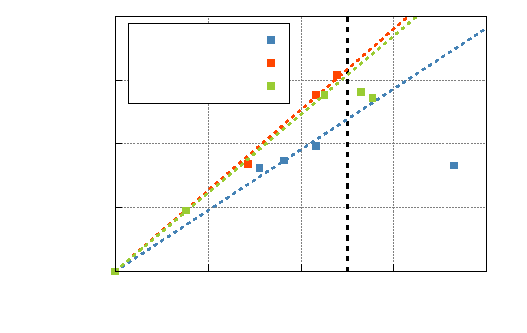
\includegraphics{5S-mass}}%
    \gplfronttext
  \end{picture}%
\endgroup

\end{minipage}
\hfill
\begin{minipage}[c]{0.48\linewidth}
\centering
\begin{tabular}{|c|c|c|c|}
\hline
K motion & Quantum	& \multicolumn{2}{c|}{Classical} \\
\hline
He density & Adiabatic	& Adiabatic & Diabatic \\
  \hline
	$\alpha$ & 0.38 & 0.50 & 0.49 \\
	\hline
	$M$ & 6.03 & 10.06 & 9.49 \\
  \hline
\end{tabular}
\end{minipage}
\vspace{0.5\baselineskip}
		\caption{Asymptotic kinetic energy as a function of excitation energy, comparison between diabatic/adiabatic classical and quantum description, and table of values for linear fit\label{fig:5S-mass}}
\end{figure}

Our model seems to work well up to 1250 K then we see some non linear effects. It is presumably due to a large amount of energy exchange with the droplet, which can no longer be described as impulsive, hard-sphere like dissociation.
We note that the classical description of K gives a higher number of neighboring helium atoms than the quantum one.
This can be surprising at first, but if we look at the ground state density profile (\citfig{fig:4S-Q-C-lsolid}), we note that the edge is smoother, so the density of neighboring atoms is lower. 
Nevertheless we are still investigating this point. 
Finally, adiabatic and diabatic descriptions seem to give similar results in classical case. 
This means that changes in density imposed by K fluctuation in equilibrium state has more or less no consequence on final kinetic energy, which is not really surprising as we are looking for asymptotic value.


